% class
\documentclass[ngerman]{scrartcl}

% input preamble
\usepackage{iftex}

% text input and font
\ifluatex  % LuaLaTeX
    \usepackage{fontspec}
    % main font automatically: Latin Modern
    \IfFontExistsTF{Fira Code}{% true branch
        \setmonofont{Fira Code}[
            Contextuals=Alternate,  % Activate the calt feature
            StylisticSet={1,3,5,8}, % fontspec docs S. 46
            CharacterVariant={16}, % fontspec docs S. 37
            Numbers={SlashedZero} % fontspec docs S. 44
        ]}{% false branch
    }
\else  % pdfLaTeX
    \usepackage[utf8]{inputenc}  % input in UTF-8
    \usepackage[T1]{fontenc}  % output in T1 fonts (west European encoding)
    \usepackage{lmodern}  % Latin modern font for main text
    \IfFileExists{fira.sty}{% true branch
        \usepackage[mono]{fira}  % Fira (not Code!) font for monospaced text
    }{% false branch
    }
\fi

% text processing
\usepackage{babel}  % language package
\usepackage[intlimits]{mathtools}  % upgrade of amsmath (automatically loaded) - \int^_ like \limits^_
\usepackage{amssymb}  % upgrade of amsfonts (American Math Society)
\usepackage{amstext}  % \text command in math environments
\usepackage{letltxmacro}  % \let command for robust macros (new sqrt)
\usepackage{chemformula}  % typeset chemical formulas


% page geometry
\usepackage{scrlayer-scrpage}  % page formatting with KOMA options
\usepackage[paper=a4paper, hmargin=3cm, vmargin=2.5cm, includehead, includefoot]{geometry}  % horizontal: 3cm, vertical: 2.5cm strict with or without headers and footers
\usepackage{tabto}  % tab stops
\NumTabs{8}  % 8 equally spaced of \textwidth tab stops



% floats
\usepackage[hypcap=false, labelfont=bf]{caption, subcaption}  % caption editing - hypcap warning with hyperref
% counter prefixed with section number and therefore reset at each section:
\counterwithin{figure}{section}
\counterwithin{table}{section}
\usepackage{float}  % for [H] (forced here) specifier
\usepackage{tabularray}  % better tables
\usepackage{caption}  % better captions


% graphical input
\usepackage{graphicx}  % input JPEG, PNG, PDF, etc.
\usepackage{pdfpages}  % input PDF as whole pages
\usepackage{lastpage}  % reference to last page
\usepackage{import} % include files from other directories


% text
\usepackage[locale=DE, uncertainty-mode=separate]{siunitx}  % SI units, German formatting - \pm stays \pm instead of ..(.)
\let\sqty\qty  % physics overrides \qty of siunitx, therefore make it available as \sqty
\usepackage{physics}  % macros for easier typesetting of physical formulas
\usepackage{icomma}  % no space after commas instead of English points) in decimal values
\usepackage{enumitem}  % better enumerating with style options
\usepackage{nicefrac}  % inline-fractions in n/d-style
\usepackage{xcolor}  % custom colors
%TU-Graz colors
\definecolor{TUred}{HTML}{e4154b}
\definecolor{TUgray}{HTML}{bcbcbc}
\usepackage{listings, scrhack}  % code display; listings in combination with KOMA
\ifluatex
    \IfFontExistsTF{Fira Code}{%
        \usepackage[verbatim]{lstfiracode}  % Fira Code in listings
        \lstset{style=FiraCodeStyle}
    }{}
\fi
\usepackage{fancyvrb}  % Verbatim environment with better options (capital V!)


% literacy
\usepackage[sorting=none, giveninits=true]{biblatex}  % defaults: backend=Biber, style=numeric
% bibliography styles: https://www.overleaf.com/learn/latex/Biblatex_bibliography_styles
% citation styles: https://www.overleaf.com/learn/latex/Biblatex_citation_styles
\usepackage{csquotes}  % better quotation - should also be used in combination with package babel (warning)
\usepackage{xurl}  % breaks links - after BibLaTeX, but before hyperref!
\usepackage[hidelinks]{hyperref}  % produces most errors, last to load


% enumerate paragraphs and subparagraphs
% depths: https://www.overleaf.com/learn/latex/Sections_and_chapters
% -1 \part{part}
%  0 \chapter{chapter}
%  1 \section{section}
%  2 \subsection{subsection}
%  3 \subsubsection{subsubsection}
%  4 \paragraph{paragraph}
%  5 \subparagraph{subparagraph}
\setcounter{secnumdepth}{3}


% KOMA setups
% header and footer
\pagestyle{scrheadings}  % KOMA style
\clearpairofpagestyles  % reset
\setkomafont{pageheadfoot}{\normalfont}  % standard font in header and footer
\setlength{\headheight}{27.2pt}  % warning
\cfoot{\pagemark{} / \pageref*{LastPage}}  % center foot - *: ref but no hyperlink
% {}: empty statement
% \ : protected space
% \,: small space
\DeclareTOCStyleEntry[linefill=\TOCLineLeaderFill]{tocline}{section}  % sections in TableOfContents with dotted lines
% source: https://tex.stackexchange.com/a/651532
\KOMAoptions{parskip=half-}  % paragraphs with half a line height space instead of indentation, last line with no special treatment


% package setups

% rewrite names (babel overwrites German with standard English names, therefore at document beginn [after everything is loaded])
\AtBeginDocument{\renewcommand{\refname}{Literaturverzeichnis}}
% others:
% \contentsname
% \listtablename
% \listfigurename

% make title in bibliography upright
\DeclareFieldFormat{title}{#1}  % https://tex.stackexchange.com/a/311837
% make size of url in bibliography smaller
\renewcommand{\UrlFont}{\footnotesize\ttfamily}  % https://tex.stackexchange.com/a/151115, https://www.overleaf.com/learn/latex/Font_sizes%2C_families%2C_and_styles


% xcolor
\definecolor{code_keyword}{HTML}{A06E9D}
\definecolor{code_string}{HTML}{AD6E3E}
\definecolor{code_comment}{HTML}{6A9955}
% \definecolor{keyword_pink}{HTML}{c678dd}
% \definecolor{vscode_bg}{HTML}{282c34}
% \definecolor{vscode_var}{HTML}{e06c75}
% \definecolor{vscode_comment}{HTML}{7f848e}
% \definecolor{vscode_constant}{HTML}{d19a66}
% \definecolor{vscode_function}{HTML}{61afe3}
% \definecolor{background_grey}{HTML}{f8f8f8}
% \definecolor{code_basic}{HTML}{D4D4D4}
% \definecolor{code_background}{HTML}{1E1E1E}

% custom siunitx units
\DeclareSIUnit{\dig}{dig}  % digits for uncertainty of electronical measurement devices
\DeclareSIUnit{\px}{px}  % pixels
\sisetup{table-align-uncertainty=true}


% listings
\lstset{
    basicstyle=\ttfamily\footnotesize,%\color{code_basic},  % \footnotesize contains \selectfont implicitly
    %backgroundcolor=\color{code_background},
    commentstyle=\color{code_comment},
    keywordstyle=\bfseries\color{code_keyword},
    numberstyle=\tiny,
    stringstyle=\color{code_string},
    breakatwhitespace=false,
    breaklines=true,
    captionpos=b,
    keepspaces=true,
    numbers=left,
    numbersep=5pt,
    showspaces=false,
    showstringspaces=false,
    showtabs=false,
    tabsize=2
}


% new sqrt
% https://en.wikibooks.org/wiki/LaTeX/Mathematics
\makeatletter
\let\oldr@@t\r@@t
\def\r@@t#1#2{%
    \setbox0=\hbox{$\oldr@@t#1{#2\,}$}\dimen0=\ht0
    \advance\dimen0-0.2\ht0
    \setbox2=\hbox{\vrule height\ht0 depth -\dimen0}%
    {\box0\lower0.4pt\box2}}
\LetLtxMacro{\oldsqrt}{\sqrt}
\renewcommand{\sqrt}[2][\ ]{\oldsqrt[#1]{#2} }
\makeatother


% own commands
% \newcommand* can't contain multiple lines
% \newcommand can
\newcommand*{\mup}[1]{\ensuremath{\text{\textup{#1}}}}  % math mode upright normal font
\newcommand*{\inkgraphics}[3][\linewidth]{\def\svgwidth{#1}\import{#2}{#3}}
\newcommand{\todo}[1]{\textbf{\textcolor{TUred}{#1\\}}}


% custom tabularray environments

% imports and setups of tabularray: {
%     expl3,
%     xparse,
%     ninecolors
%     \hypersetup{pdfborder={0 0 0}}
% }

% additionally loaded libraries:
% diagbox
% varwidth
% booktabs
% counter

\UseTblrLibrary{amsmath}  % +array, +matrix, +bmatrix, +Bmatrix, +pmatrix, +vmatrix, +Vmatrix and +cases like tabularray with graphical options
\UseTblrLibrary{siunitx}  % siunitx suited for tabularray
\UseTblrLibrary{diagbox}  % table cells with diagonal lines, suited for tabularray
\UseTblrLibrary{varwidth}  % measure cell width
\UseTblrLibrary{booktabs}
\UseTblrLibrary{counter}


% custom tabularray environments:

% info:
% colcycle: https://github.com/lvjr/tabularray/issues/74
% guard: https://github.com/lvjr/tabularray/issues/175#event-6567229210

% guard S columns if latest feature ={guard} is not yet available
\newcommand*{\SiGuard}[1]{{#1}}

% standard environment
\SetTblrInner{
    hlines,
    vlines,
    columns={
            halign=c,
            valign=m,
        },
    measure=vbox,
}

% X columns
\NewTblrEnviron{tblrx}
\SetTblrInner[tblrx]{
    hlines,
    vlines,
    columns={
            halign=c,
            valign=m,
            co=1,  % coefficient of width for expendable columns (X columns)
        },
    width=\linewidth,
    vspan=minimal,
    measure=vbox,
}

% -X columns
\NewTblrEnviron{tblr-x}
\SetTblrInner[tblr-x]{
    hlines,
    vlines,
    columns={
            halign=c,
            valign=m,
            co=-1,  % shrinks X column down to natural width
        },
    width=\linewidth,
    vspan=minimal,
    measure=vbox,
}

% no hline and vline left and on top of first cell
\NewTblrEnviron{tblr_omit_first_cell}
\SetTblrInner[tblr_omit_first_cell]{
    hlines,
    vlines,
    columns={
            halign=c,
            valign=m,
        },
    hspan=even,
    vspan=minimal,
    %
    hline{1}={1}{white},  % first row, only first cell
    vline{1}={1}{white},
    measure=vbox,
}

% longtblr
\DefTblrTemplate{conthead-text}{default}{(Fortsetzung)}  % default: define and set at the same time
\DefTblrTemplate{contfoot-text}{default}{Fortsetzung auf nächster Seite}
\SetTblrStyle{caption-tag}{font=\bfseries}  % caption tag bold
\SetTblrInner[longtblr]{
    hlines,
    vlines,
    columns={
            halign=c,
            valign=m,
        },
    measure=vbox,
}

% longtblr - to adjust width of caption 
\DefTblrTemplate{firsthead}{default}{\addtocounter{table}{-1}\captionof{table}[\InsertTblrText{entry}]{\InsertTblrText{caption}}}
\DefTblrTemplate{middlehead,lasthead}{default}{\addtocounter{table}{-1}\captionof{table}[]{\InsertTblrText{caption}~(Fortsetzung)}}
%info ADD this to a local environment around the longtblr: \captionsetup{format=plain,labelfont=bf,font=small,  width=\linewidth}

% manual header
\ihead{Compton Effekt \&\newline Röntgenfluoreszenzanalyse}  % inner (left) head
\chead{\textsc{Wachmann} Elias (12004232)\\\textsc{Zach} Andreas (12004790)}  % center head
\ohead{17.03.2023}  % outer (right) head

\addbibresource{Compton.bib}



\begin{document}

%%%%Title Page %%%%
\begin{titlepage}
    \centering
    
\includegraphics[width=0.5\textwidth]{../../99_Misc/Logo_KF.pdf}\par\vspace{0.8cm}
    {\scshape\LARGE{Karl-Franzens-Universität Graz}\par}
    {\scshape\LARGE{Institut für Physik}\par}
    \vspace{1cm}
    {\scshape\Large{23S PHY.L02UB Fortgeschrittenenpraktikum 2}\par}
    678 Bachelorstudium Physik, UG2002/2021W\par
    \vspace{1.5cm}
    {\huge\bfseries I. Compton Effekt \& Röntgenfluoreszenzanalyse\par}
    \vspace{2cm}
    \begin{table}[H]
        \centering
        \begin{tabular}{c c c}
            \Large Wachmann Elias &  & \Large Zach Andreas \\
            \Large 12004232       &  & \Large 12004790     \\
            \multicolumn{3}{c}{Gruppe 12}
        \end{tabular}
    \end{table}
    \vfill
    \Large Betreut von\par
    Thomas Georg \textsc{Boné}, BSc MSc
    \vfill
    % Bottom of the page
    {\large 17.03.2023\par}
\end{titlepage}
%%%%

\clearpage
\tableofcontents
\newpage

\section[Aufgabenstellung]{Aufgabenstellung \cite{ref:angabe_compton,ref:angabe_roentgen}}
\label{sec:aufgabenstellung}

Die vorliegende Laboreinheit teilt sich in zwei Teilversuche:

\begin{itemize}
    \item \textbf{Compton-Effekt}
          \begin{itemize}
              \item Aufnahme des Primärspektrums und Energiekalibrierung des Detektors
              \item Bestimmung der Energie als Funktion des Streuwinkels
          \end{itemize}
    \item \textbf{Röntgenfluoreszenzanalyse}
          \begin{itemize}
              \item Aufnahme und Kalibrierung eines Röntgenenergiespektrums
              \item Zeigen der Gültigkeit des Moseley'schen Gesetzes Ermitteln der jeweiligen Abschirmkonstanten der K-Linien
              \item Analyse der Zusammensetzung mehrerer unbekannter Proben
          \end{itemize}
\end{itemize}


\section{Grundlagen}
\label{sec:grundlagen}

\subsection[Compton-Effekt]{Compton-Effekt \cite{ref:angabe_compton}}
\label{subsec:grundlagen_compton}

Der Compton-Effekt beschreibt die Streuung von Photonen an freien Elektronen und ist ein wichtiger Prozess in der Wechselwirkung von Licht und Materie. Er wurde erstmals von Arthur Compton im Jahr 1923 entdeckt.
%
\begin{figure}[!h]
    \centering
    \begin{samepage}
        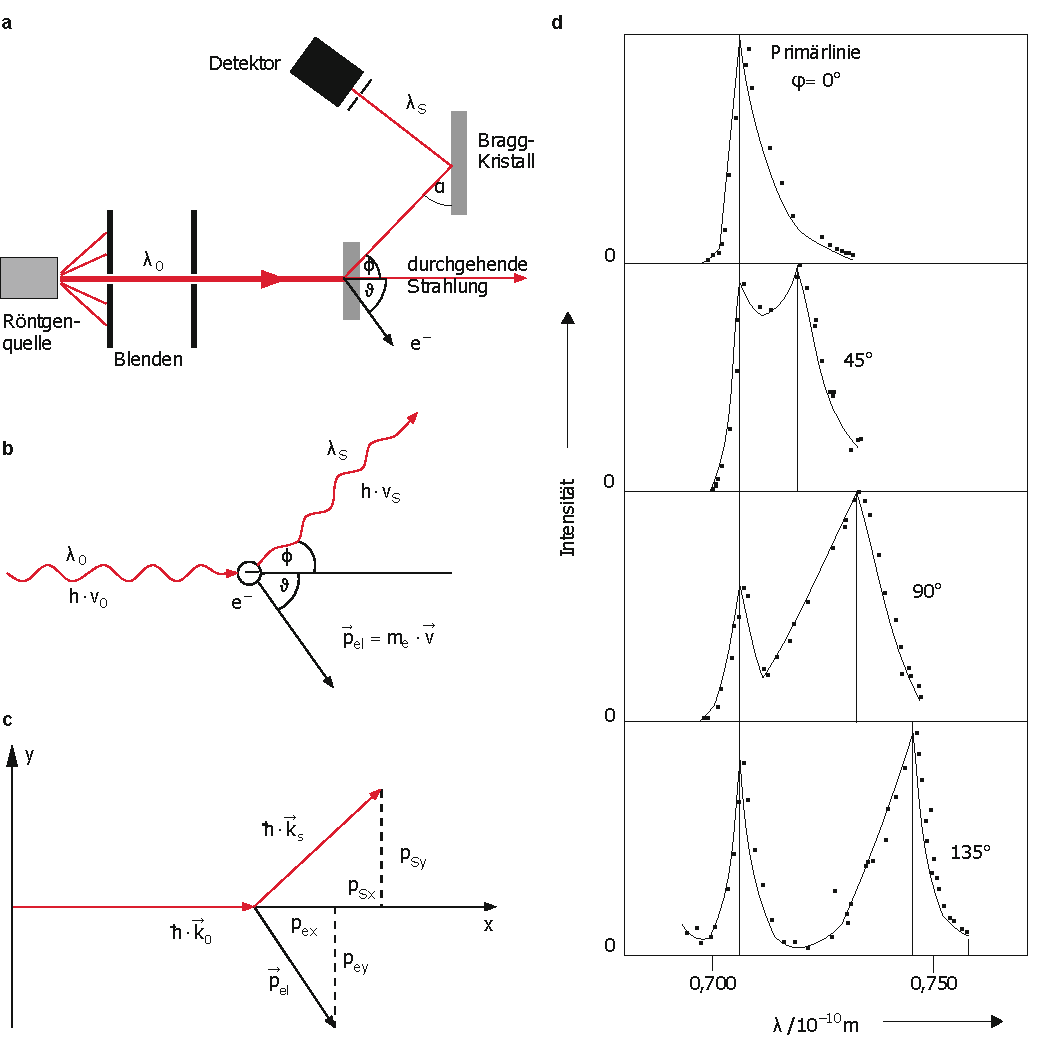
\includegraphics[width=0.8\linewidth]{fig/compton_complete.pdf}
        \caption[Compton-Effekt]{Comptoneffekt: \textbf{(a)} Experiment; \textbf{(b)} Schema; \textbf{(c)} Vektordiagramm; \textbf{(d)} Wellenlängen $\lambda_S$ als Funktion des Streuwinkels für die Streuung der K$_\alpha$-Strahlung
            von \ch{Mo} in Graphit gemessen 1923 von \textit{Compton}. Quelle: \cite{ref:demtroeder}}
        \label{fig:compton_effekt_demtroeder}
    \end{samepage}
\end{figure}
%
Bestrahlt man beliebiges Material mit Röntgenstrahlung der Wellenlänge $\lambda_0$, so findet man in der Streustrahlung außer der erwarteten Wellenlänge $\lambda_0$ (aufgrund elastischer Streuung) auch Anteile mit größerer Wellenlänge $\lambda_S > \lambda_0$ (aufgrund elastischer Stöße). Dies lässt sich wie folgt erklären (siehe auch \autoref{fig:compton_effekt_demtroeder}):

Wenn ein Photon auf ein Elektron trifft, kann es idealisiert gesehen elastisch gestreut oder gestoßen werden. Im Falle des Stoßprozesses gibt es einen Teil seiner Energie und Impuls an das Elektron ab. Durch diesen Impulstransfer ändert sich die Richtung und kinetische Energie des Photons.
Aufgrund des Zusammenhangs der Energie $E$ eines quantenmechanischen Teilchens mit seiner Frequenz $\nu$ (bzw. Wellenlänge $\lambda$)
\begin{equation}
    \label{eq:energie_frequenz_wellenlaenge}
    E = h \nu = h \frac{c}{\lambda}
\end{equation}
über das Planck'sche Wirkungsquantum $h$ wird ersichtlich, dass sich beim Verlust von Energie auch die Frequenz verringern bzw. die Wellenlänge des Teilchens erhöhen muss. Der Impuls des Photons genügt folgenden Zusammenhängen:
\begin{align}
    \vb*{p}     & = \hbar \vb*{k} \label{eq:impuls}            \\
    ||\vb*{p}|| & = \frac{h}{\lambda} \label{eq:impuls_betrag}
\end{align}
wobei $\vb*{k}$ der Wellenvektor des Photons ist und $\hbar$ das reduzierte Planck'sche Wirkungsquantum.
In relativistischer Betrachtung lautet der Energiesatz somit:
\begin{equation}
    \label{eq:energiesatz_relativistisch}
    E_{\text{kin}} = \frac{m_0c^2}{\sqrt{1-\frac{v^2}{c^2}}} - m_0 c^2
\end{equation}
Für den Impuls folgt:
\begin{equation}
    \label{eq:impuls_beziehung}
    \hbar \vb*{k}_0 = \hbar \vb*{k}_S + \frac{m_0 \vb*{v}}{\sqrt{1-\frac{v^2}{c^2}}}
\end{equation}
Daraus folgt:
\begin{equation}
    \label{eq:Delta_nu}
    \Delta \nu = \nu_0 - \nu_S = \frac{h}{m_0 c^2} \nu_0 \nu_S (1-\cos(\varphi))
\end{equation}
Und die Compton-Streuformel:
\begin{equation}
    \label{eq:}
    \lambda_S - \lambda_0 = 2 \underbrace{\frac{h}{m_0 c}}_{\mathclap{\text{Compton-Wellenlänge}}} \sin^2\left(\frac{\varphi}{2}\right)
\end{equation}
Führt man diese Formeln zusammen, erhält man die Energie der gestreuten Strahlung $E_S$
\begin{equation}
    \label{eq:energie_gestreute_strahlung}
    E_S = \frac{E_0}{1 + \frac{E_0}{m_0 c^2} (1-\cos(\varphi))}
\end{equation}

Die Wellenlängenänderung des Photons hängt also vom Streuwinkel und der Energie des Photons ab. Je größer der Streuwinkel, desto größer ist die Wellenlängenverschiebung des Photons. Die Energie des Photons ist proportional zur Frequenz und umgekehrt proportional zur Wellenlänge. Daher führt der Compton-Effekt zu einer Abnahme der Energie des Photons und einer Zunahme seiner Wellenlänge.


\subsection[Röntgenfluoreszenzanalyse]{Röntgenfluoreszenzanalyse \cite{ref:angabe_roentgen}}
\label{subsec:grundlagen_roentgen}

Werden Atome mit hochenergetischer Röntgenstrahlung bestrahlt, so können durch die zugeführte
Energie Elektronen aus den inneren Schalen herausgeschlagen werden. Die Lücken in den inneren
Schalen füllen sich dann durch Elektronen aus äußeren Schalen auf. Dabei verlieren diese Elektronen
Energie, die wiederum in Form von Röntgenstrahlung emittiert wird. Dieses Phänomen wird als
\textit{Röntgenfluoreszenz} bezeichnet. Werden Elektronen aus der innersten Schale (K-Schale)
herausgeschlagen, so entsteht das sogenannte K-Spektrum (die K-Spektralserie). Der griechische Buchstabe
einer Übergangslinie codiert aus einer wie viel energetisch höheren Schale das auffüllende Elektron stammt.
Springt das Elektron nur eine Schale nach unten (also in diesem Fall von L nach K), so schreibt man ein $\alpha$.
Bei einem Sprung von der zweithöheren Schale (M nach K) schreibt man ein $\beta$ usw.
Analog entsteht das L-Spektrum,
wenn Elektronen auf die 2. Schale (L-Schale) zurückfallen. Die Energie der emittierten Strahlung einer
Schale ist abhängig von der Kernladungszahl (Moseley'sches Gesetz).
\begin{equation}
    \label{eq:moseley}
    \sqrt{\frac{E}{R_y}} = (Z-\sigma_{2,1})\sqrt{n_1^{-2}-n_2^{-2}}
\end{equation}
Dabei beschreiben $n_1$ und $n_2$ die Hauptquantenzahlen der Schalen beim Übergang von $n_2$ nach $n_1$, $\sigma_{2,1}$ die mittlere Abschirmkonstante bei diesem Übergang, $Z$ die Kernladungszahl, $R_y=\SI{13,6}{eV}$ die angepasste Rydberg-Frequenz und $E$ die Energie der Röntgenstrahlung. Für die K$_\alpha$-Linien leichterer Elemente ($Z<30$) ist die Abschirmkonstante $\sigma_{2,1}=1$ und somit
\begin{equation}
    \label{eq:moseley_einfach}
    \sqrt{\frac{E}{R_y}} = (Z-1)\sqrt{\frac{3}{4}}
\end{equation}
Dies ermöglicht die eindeutige
Bestimmung der Kernladungszahl eines Elements und war historisch ein wichtiger Bestandteil für die
Vervollständigung des Periodensystems. Jedes Element (mit jeweils einer anderen Kernladungszahl)
emittiert Röntgenstrahlung mit einer charakteristischen Energie. Die Energie ist dabei praktisch
unabhängig von der Bindungsform des Elements, weil die inneren Elektronen nicht zur
chemischen Bindung beitragen. So kann durch Röntgenfluoreszenzanalyse die Zusammensetzung von
Materialien bestimmt werden, auch wenn diese in chemisch verschiedenen Formen vorliegen. Das
Röntgenfluoreszenzspektrum einer homogenen Probe mit mehreren Komponenten ist in erster
Näherung eine Addition der Einzelspektren. Deshalb kann mit dieser Methode die Zusammensetzung
von beliebigen Proben qualitativ bestimmt werden. Dafür werden zunächst alle im
Fluoreszenzspektrum vorhandenen Signale den Elementen zugeordnet. Dies geschieht mithilfe von
Tabellenwerten für die Energien der charakteristischen Linien. Für die Zuordnung wird auch das
Muster jeder Spektralserie berücksichtigt: Zu jeder K$_\alpha$-Linie gehört eine K$_\beta$-Linie mit ca. fünf- bis zehnfach
geringerer Intensität.


\subsection{Unsicherheitsanalyse}
\label{subsec:unsicherheitsanalyse}

Die Fehlerfortpflanzung der berechneten Werte basiert auf der Größtunsicherheitsmethode nach Gauß. Um diese Berechnungen zeiteffizient durchführen zu können, wird für jeden Unterpunkt der Laborübung ein Skript in \texttt{Python} implementiert. Kernstück dessen ist das package \texttt{uncertainties} \cite{ref:uncertainties}, das intern die Fehlerfortpflanzung berechnet. Gerundet wird nach den Angaben des Skriptums der Lehrveranstaltung \enquote{Einführung in die physikalischen Messmethoden} \cite{ref:messmethoden}.



\section{Geräteliste}
\label{sec:geraeteliste}

Für den praktischen Aufbau und die Messungen der geforderten Größen wurden die in \autoref{tab:geraeteliste} aufgelisteten Geräte und Hilfsmittel verwendet.
%
\begin{table}[H]
    \centering
    \begin{samepage}
        \caption[Geräteliste]{Verwendete Geräte und wichtige Materialien}
        \label{tab:geraeteliste}
        \begin{tblrx}{cells={font=\footnotesize}}
            Gerät                      & Hersteller & Modell                   & Inventar-Nr. \\
            Röntgengerät               & Leybold    & 554 800                  & 310082130000 \\
            Messwerterfassungsmodul    & Leybold    & (Sensor-CASSY 2) 524 013 & -            \\
            Proben                     & -          & -                        & -            \\
            Messwerterfassungssoftware & Leybold    & CASSY Lab 2              & -            \\
        \end{tblrx}
    \end{samepage}
\end{table}
%
\paragraph{Anmerkung zu den Unsicherheiten:} Zur Unsicherheitsangabe werden die jeweiligen Unsicherheitsmaße der Geräte, welche aus den Datenblättern (sofern vorhanden) entnommen werden, verwendet. Für die analogen Messgeräte wird eine kombinierte Ablese- und Messunsicherheit von $\pm\SI{1}{Skalenstrich}$ verwendet.

Alle Teilversuche wurden bei einer Umgebungstemperatur von \SI{24(1)}{\celsius} einem Luftdruck von \SI{1000(10)}{\hecto\pascal} und einer relativen Luftfeuchtigkeit von \SI{33(1)}{\percent} durchgeführt.



\section{Versuchsaufbau}
\label{sec:aufbau}

Beide Teilversuche benötigen beinahe den identen Aufbau aus Röntgengerät, Messwerterfassungsmodul (Sensor-CASSY) und PC. Die minimalen Unterschiede werden in den nachfolgenden Unterabschnitten erläutert. Ansonsten folgen beide Aufbauten der folgenden Beschreibung:

Das Röntgengerät ist an seinem SIGNAL-OUT-Ausgang mittels eines Koaxialkabels mit dem INPUT-Eingang des Messwerterfassungsmoduls verbunden. Das Messwerterfassungsmodul ist mit einem USB-B-Kabel mit dem PC verbunden, welcher über die Software CASSY Lab das Modul steuert. Das Röntgengerät selbst weist zwei Räume auf, die jeweils mit einer Bleiglasscheibe verschlossen sind: den Röntgenraum und den Experimentierraum. Diese Räume sind durch eine kreisrunde Öffnung miteinander verbunden. In diese Öffnung ist ein kreisrunder Kollimator eingeführt. Im Experimentierraum befindet sich ein Röntgenenergiedetektor. Die Position dessen ist manuell so gewählt, dass der Sensor bei einer Drehung um \SI{150}{\degree} zur Nullstellung nicht mit dem Röntgenstrahl -- geschweige denn mit dem Kollimatorrohr -- kollidiert.

Relevante Parameter für den Messvorgang sind folgendermaßen eingestellt: Für die Glühkathode des Röntgengeräts ist an jenem eine Spannung von \SI{30}{kV} eingestellt, die Emissionsstromstärke beträgt generell \SI{1}{mA}. In der PC-Software CASSY Lab ist der Parameter \textit{Vielkanalmessung} auf 512 Kanäle eingestellt und negative Pulse sind aktiviert, gemessen wird mit einer Torzeit von \SI{300}{s}.


\subsection{Compton-Effekt}
\label{subsec:aufbau_compton}

Für den Teilversuch zum Compton-Effekt ist in der Software CASSY Lab der Verstärkungsfaktor auf -4 gestellt. Zusätzlich ist auf das zum Röntgenraum zeigende Ende des Kollimators ein \ch{Zr}-Filter gesteckt.


\subsection{Röntgenfluoreszenzanalyse}
\label{subsec:aufbau_fluoreszenz}

Für den Teilversuch zur Röntgenfluoreszenzanalyse ist in der Software CASSY Lab der Verstärkungsfaktor auf \num{-2.5} gestellt.



\section{Versuchsdurchführung}
\label{sec:durchfuehrung}

\subsection{Compton-Effekt}
\label{subsec:durchfuehrung_compton}

Der Aufbau zum Teilversuch Compton-Effekt wird ordnungsgemäß, wie in \autoref{sec:aufbau} beschrieben, hergestellt.

\paragraph{Primärspektrum und Energiekalibrierung}
Zuallererst muss der Röntgenenergiedetektor mithilfe eines bereits bekannten Spektrums kalibriert werden. Dazu wird auf das zum Experimentierraum zeigende Ende des Kollimators zusätzlich eine Abschwächblende gesteckt. Für die Energiekalibrierung wird darüberhinaus die Stromstärke von \SI{1}{mA} auf (vorläufig) \SI{0.05}{mA} reduziert. Der Sensorarm soll in Nullstellung gebracht werden, der Motor des Arms ist jedoch nicht präzise auf einen tatsächlichen Winkel von \SI{0}{\degree} zur Röntgenstrahlaustrittsöffnung kalibriert, daher muss der tatsächliche Nullpunkt manuell gefunden werden. Bei direkter Einstrahlung (Winkel von \SI{0}{\degree}) muss der Sensor die höchste Aktivität detektieren, deswegen wird in \SI{0.1}{\degree} Schritten vom voreingestellten (tatsächlich jedoch verschobenen) Nullpunkt weg mit einer Torzeit von \SI{10}{s} nach der höchsten Zerfallsanzahl gesucht. Die Messwerte lassen auf einen Offset von \SI{-1.6}{\degree} schließen, eine erneute Messreihe mit einer erhöhten Torzeit auf \SI{60}{s} um diese Sensorstellung herum bestätigt die Vermutung. Somit ist die tatsächlich ermittelte Nullstellung
\[\varphi_0 = \SI{-1.6}{\degree}.\]
Nun wird mit einer verringerten Torzeit von \SI{10}{s} eine passende Emissionsstromstärke gewählt, sodass die Zerfallsrate etwas über \SI{200}{\per\second} liegt. Dies ist bei einer Stromstärke von
\[I_0=\SI{0.14}{mA}\]
der Fall.

Nachdem nun die Ausgangsstellung mit $\varphi_0 = \SI{-1.6}{\degree}$ und $I_0=\SI{0.14}{mA}$ ermittelt worden ist, wird das Primärspektrum der Röntgenröhre aufgenommen. Gemessen wird mit der ursprünglich beschriebenen Torzeit von \SI{300}{s}. Nachdem das Spektrum von der Software erfasst worden ist, dienen die L$_\alpha$-Linie von \ch{Au} (bei \SI{9.71}{keV}) und die K$_\alpha$-Linie von \ch{Mo} (bei \SI{17.44}{keV}) als Referenz zur Kalibrierung der Energieskala. Dabei werden die Positionen der Peakschwerpunkte des Primärspektrums diesen Energien zugeordnet.

\paragraph{Streuspektren}
Nach das Messgerät nun kalibriert worden ist, wird die Abhängigkeit des Streuspektrums vom Winkel untersucht. Hierfür wird die Abschwächblende wieder vom Kollimator genommen und der Targethalter samt Targettsich am Goniometer im Experimentierraum montiert. Als Target kommt eine Plexiglas-Probe zum Einsatz. Der Emissionsstrom wird nun wieder, wie ursprünglich angegeben, auf \SI{1}{mA} erhöht. Der Winkel des Targethalters (Targetwinkel) wird auf \SI{20}{\degree} gestellt, während der Sensorwinkel im Zuge des Experiments laufend verstellt wird. Begonnen wird mit \SI{28.4}{\degree} ($\SI{30}{\degree} - \SI{1.6}{\degree}$), das emittierte Spektrum wird aufgenommen. Dieser Vorgang wird für die folgenden Winkel wiederholt:
\begin{itemize}
    \item \SI{43.4}{\degree}
    \item \SI{58.4}{\degree}
    \item \SI{73.4}{\degree}
    \item \SI{88.4}{\degree}
    \item \SI{103.4}{\degree}
    \item \SI{118.4}{\degree}
    \item \SI{133.4}{\degree}
    \item \SI{148.4}{\degree}
\end{itemize}
Jede Messreihe wird als \texttt{.csv}-Datei abgespeichert.


\subsection{Röntgenfluoreszenzanalyse}
\label{subsec:durchfuehrung_fluoreszenz}

\paragraph{Kalibrierung}
Zuerst wird das Gerät wieder kalibriert. Dazu werden zuerst manuell im Experimentierraum die Abstände zwischen Spaltblende des Kollimators und Drehachse sowie zwischen Drehachse und Eintrittsöffnung des Röntgenenergiedetektors jeweils auf \SIrange{5}{6}{cm} eingestellt. Zur Kalibrierung sollte ein verzinktes Eisenblech verwendet werden, dieses ist jedoch nicht auffindbar gewesen. Stattdessen haben sich jedoch Elementarproben von \ch{Fe} und \ch{Zn} im Probenvorrat befunden, sodass diese nacheinander anstelle des verzinkten Eisenblechs verwendet worden sind. Der Sensorwinkel wird auf \SI{88.4}{\degree} (Offset-bereinigt) gestellt, der Targetwinkel auf \SI{45}{\degree}. In der Software CASSY Lab gelten nun die Parameter aus \autoref{subsec:aufbau_fluoreszenz}.

Nachdem beide Spektren gemessen worden sind, wird die Energieskala diesmal mithilfe der K$_\alpha$-Linien von \ch{Fe} (\SI{6,40}{keV}) und \ch{Zn} (\ch{8,64}{keV}) kalibriert.

\paragraph{Moseley'sches Gesetz}
Zur anschließenden Verifizierung des Moseley'schen Gesetzes werden nun die Spektren folgender Elementarproben aufgenommen und anschließenden als \texttt{.csv}-Datei abgespeichert:
\begin{itemize}
    \item Titan (\ch{Ti})
    \item Eisen (\ch{Fe})
    \item Nickel (\ch{Ni})
    \item Kupfer (\ch{Cu})
    \item Zink (\ch{Zn})
    \item Zirconium (\ch{Zr})
    \item Molybdän (\ch{Mo})
    \item Silber (\ch{Ag})
\end{itemize}

\paragraph{Unbekannte Proben}
Abschließend werden drei unbekannte Proben (siehe \autoref{fig:unbekannte_proben}) am Targethalter platziert. Deren Spektren werden wieder aufgenommen, für die unbekannte Probe 1 (eine goldgelbe Platte mit Beschriftung \enquote{3}) nach wie vor mit einer Messzeit von \SI{300}{s}, für die unbekannte Probe 2 (eine schwarze unbeschriebene Platte) und die unbekannte Probe 3 (ein gold-silberner Ring eines Experimentierenden) wird die Messzeit auf \SI{10}{s} reduziert. Die Spektren werden als \texttt{.csv}-Datei abgespeichert. Die dritte Probe gestaltet sich schwieriger korrekt zu platzieren, da der Ring keine plane Oberfläche aufweist, von welcher im richtigen Winkel zum Sensor reflektiert würde. Deswegen wird, um möglichst dem Setting der Probenplatten gleichzukommen, der Targetwinkel auf \SI{15.3}{\degree} verstellt.
%
\begin{figure}[H]
    \centering
    \begin{samepage}
        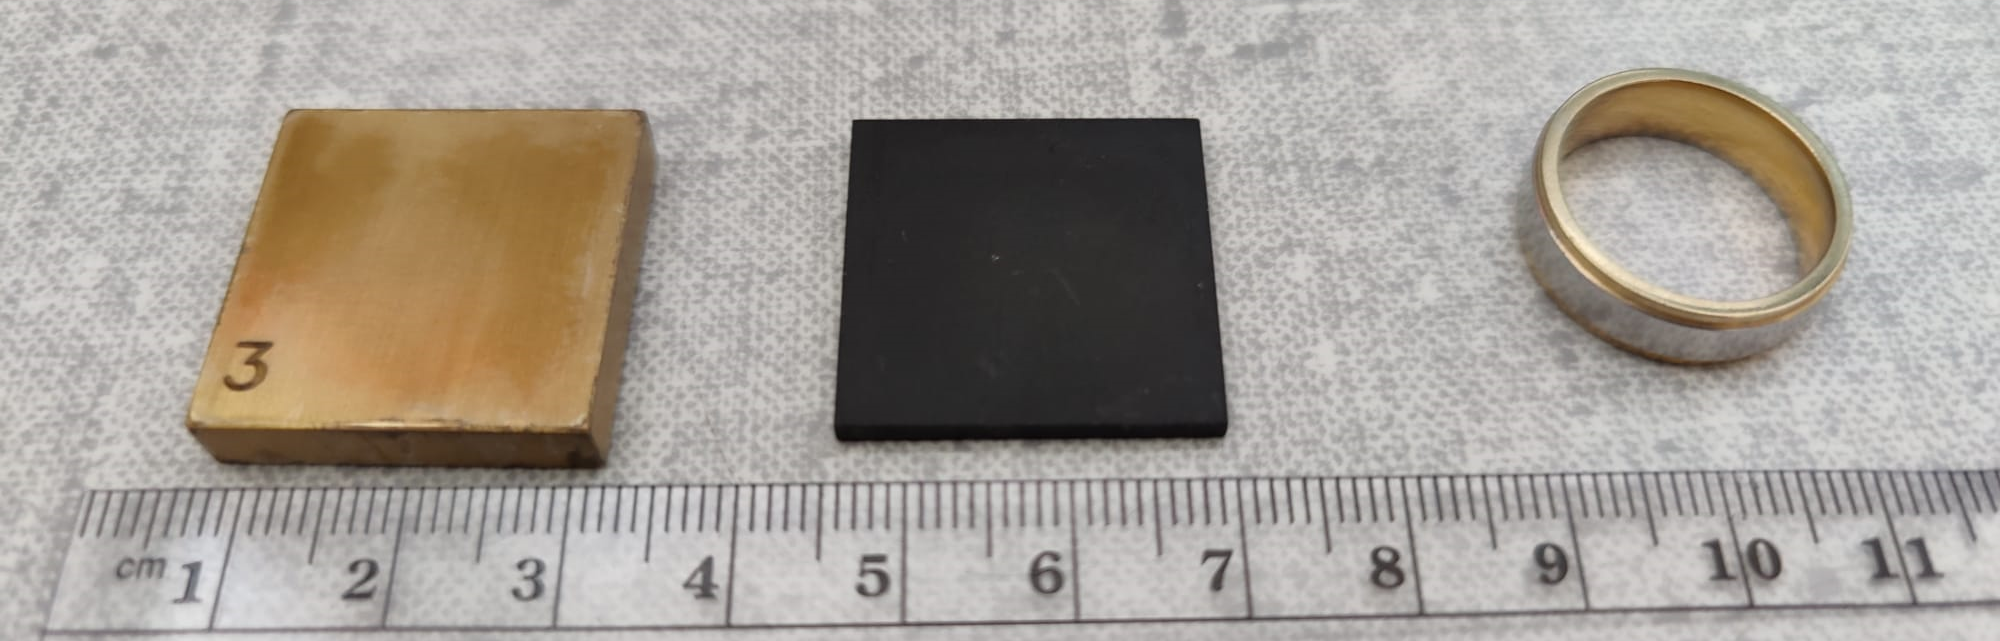
\includegraphics[width=\linewidth]{fig/unbekannt.png}
        \caption[Unbekannte Proben]{Unbekannte Proben verwendet zur Röntgenfluoreszenzanalyse.}
        \label{fig:unbekannte_proben}
    \end{samepage}
\end{figure}



\section{Auswertung}
\label{sec:auswertung}

\subsection{Compton-Effekt}
\label{subsec:auswertung_compton}

Die gegeben der Beschreibung in \ref{subsec:durchfuehrung_compton} erhaltenen Messwerte in \texttt{.csv}-Form werden nun für die jeweiligen Stellungen des Messarms in \autoref{fig:compton_uebersicht1} und \autoref{fig:compton_uebersicht2} dargestellt.
%
\begin{figure}[H]
    \centering
    \begin{tabular}{cc}
        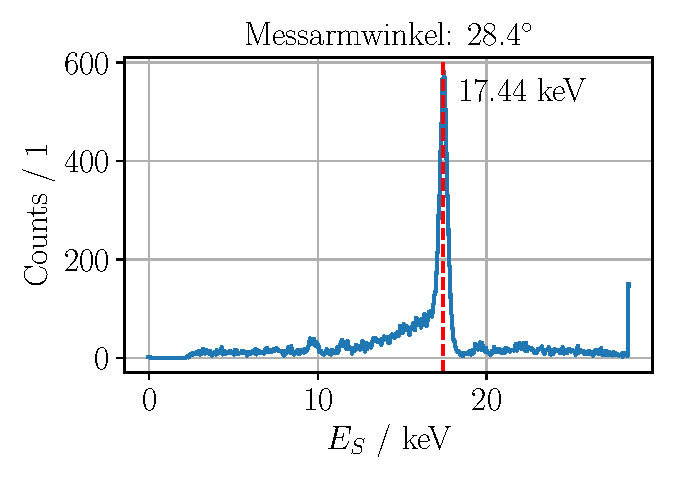
\includegraphics[width=0.48\textwidth]{../plots/energie_spektren_1.pdf} &
        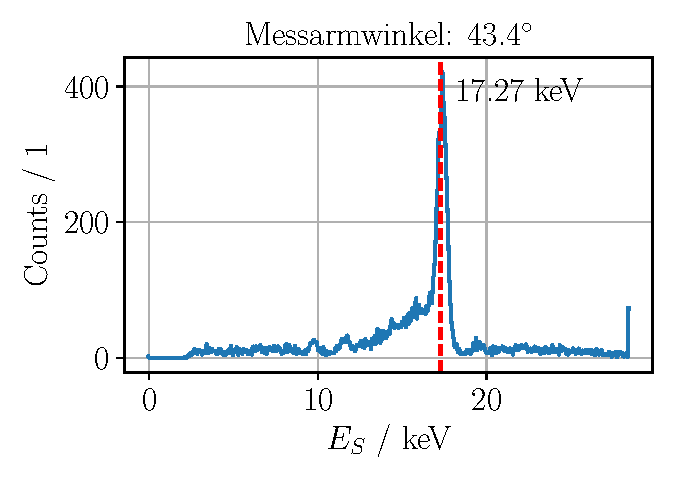
\includegraphics[width=0.48\textwidth]{../plots/energie_spektren_2.pdf}   \\
        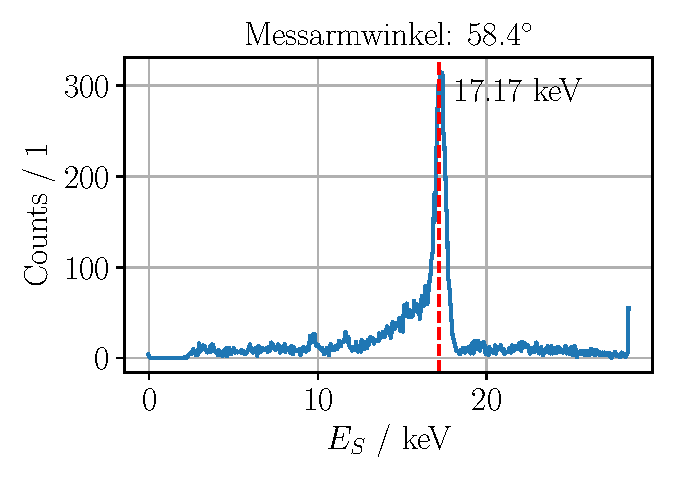
\includegraphics[width=0.48\textwidth]{../plots/energie_spektren_3.pdf} &
        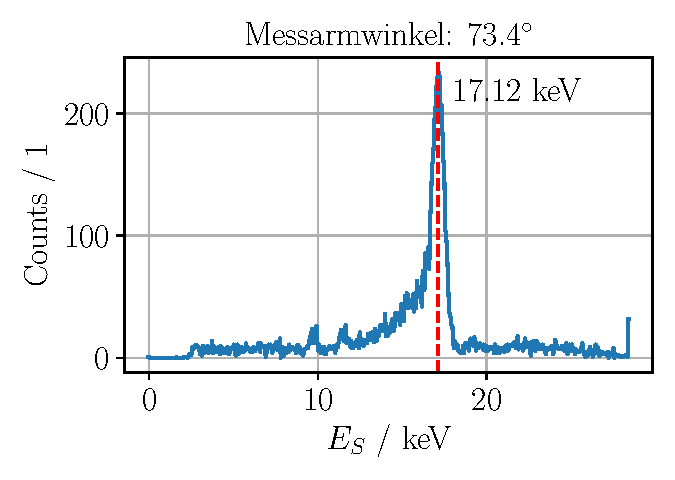
\includegraphics[width=0.48\textwidth]{../plots/energie_spektren_4.pdf}   \\
        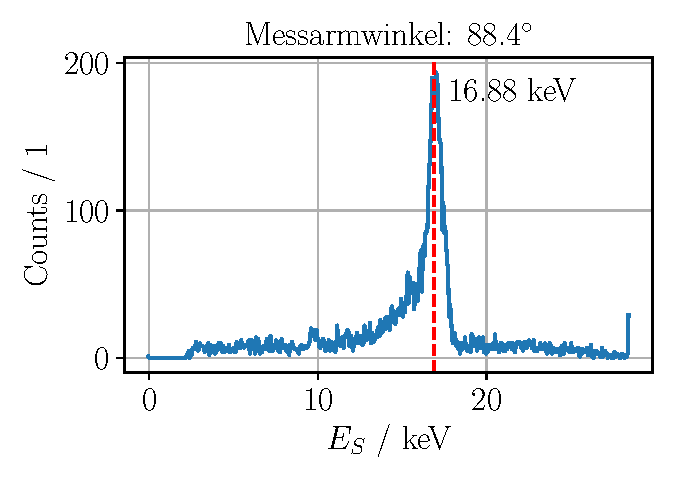
\includegraphics[width=0.48\textwidth]{../plots/energie_spektren_5.pdf} &
        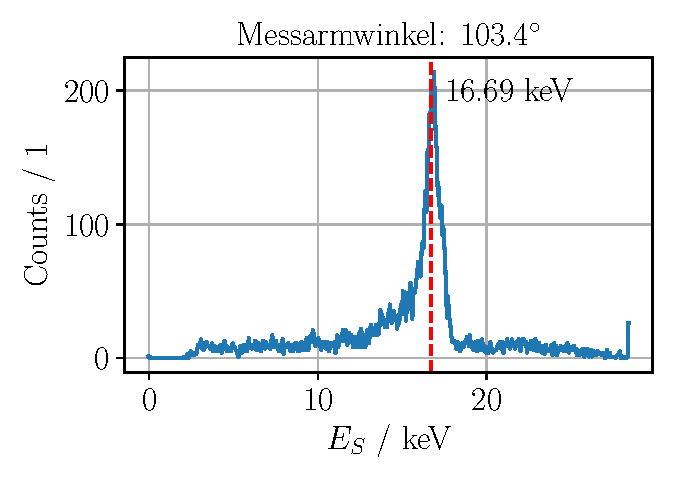
\includegraphics[width=0.48\textwidth]{../plots/energie_spektren_6.pdf}   \\
        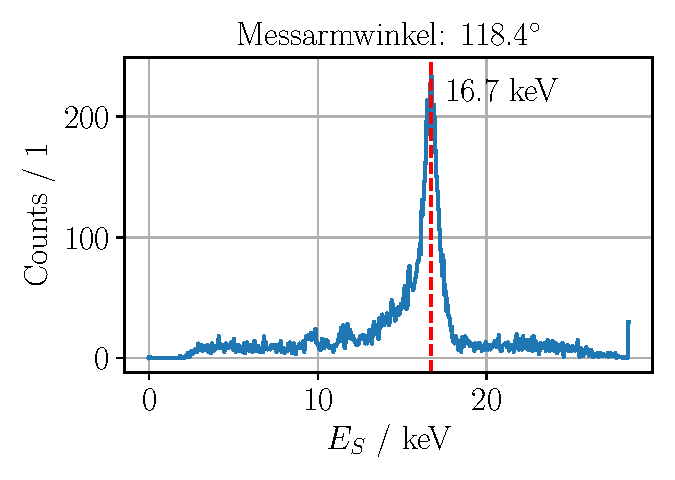
\includegraphics[width=0.48\textwidth]{../plots/energie_spektren_7.pdf} &
        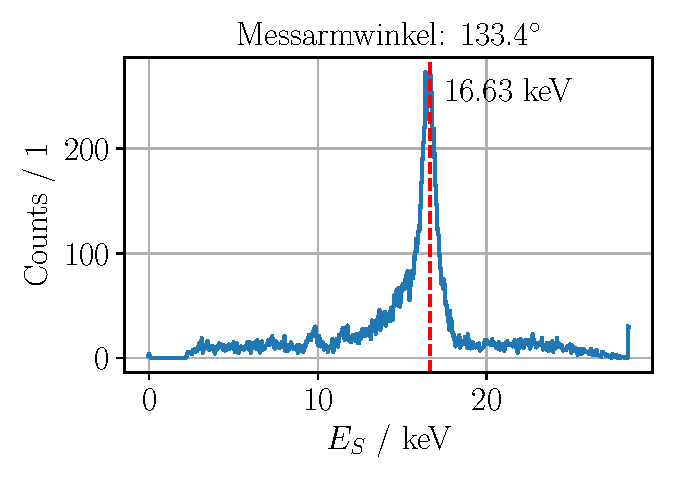
\includegraphics[width=0.48\textwidth]{../plots/energie_spektren_8.pdf}   \\
    \end{tabular}
    \caption{Messwerte bei gegebenem Winkel des Messarms \autoref{tab:compton_uebersicht1} (1)} % wohin soll diese Referenz gehen?
    \label{fig:compton_uebersicht1}
\end{figure}
%
\begin{figure}[H]
    \centering
    \begin{samepage}
        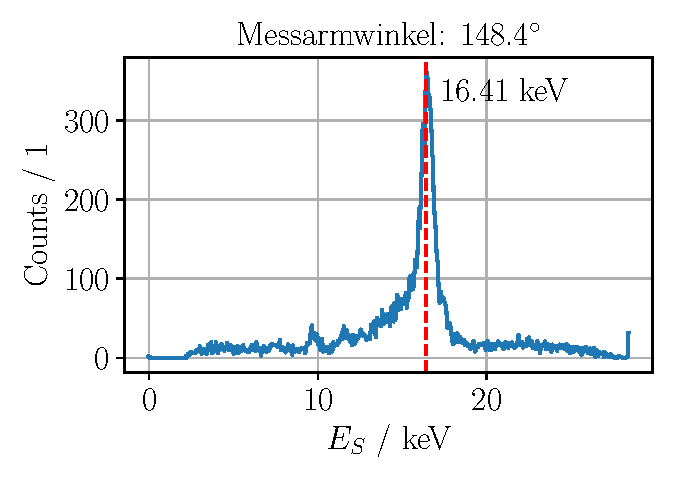
\includegraphics[width=0.5\textwidth]{../plots/energie_spektren_9.pdf}
        \caption{Messwerte bei gegebenem Winkel des Messarms \autoref{tab:compton_uebersicht2} (2)} % wohin soll diese Referenz gehen?
        \label{fig:compton_uebersicht2}
    \end{samepage}
\end{figure}
%
Anschließend werden die jeweiligen Maxima in den Daten ausgewertet, diese ergeben sich zu den nachfolgenden Werten in \autoref{tab:energy_compton}.
%info Probenhalter wird ohne Winkelfehler angenommen, daher ist der erste Winkel zwischen Probe und Messgerät 10° 
\begin{table}[H]
    \centering
    \begin{samepage}
        \caption[Messwerte Compton-Energiemaxima]{Energie $E_S$ der Countmaxima der Compton-Streuung (mit $\Delta E_S=\SI{0.2}{\kilo\electronvolt}$) für verschiedene Winkel $\varphi$ (mit $\Delta \varphi=\SI{0.1}{\degree}$) des Messarms. Zudem ist der Winkel zur Probenoberfläche $\vartheta$ (mit $\Delta \vartheta=\SI{0.1}{\degree}$) angegeben. Der Winkel des Probentisches mit $\varPsi$ wird bei \SI{20}{\degree} konstant gehalten.}
        \label{tab:energy_compton}
        \begin{tblr}{colspec={S[table-format=3.1] S[table-format=2.1]S[table-format=2.1]}, row{1}={guard}}
            $\varphi$ / \unit{\degree} & $E_S$ / \unit{\kilo\electronvolt} & $\vartheta$ / \unit{\degree} \\
            28.4                       & 17.4                              & 6.8                          \\
            43.4                       & 17.3                              & 21.8                         \\
            58.4                       & 17.2                              & 36.8                         \\
            73.4                       & 17.1                              & 51.8                         \\
            88.4                       & 16.9                              & 66.8                         \\
            103.4                      & 16.7                              & 81.8                         \\
            118.4                      & 16.7                              & 96.8                         \\
            133.4                      & 16.6                              & 111.8                        \\
            148.4                      & 16.4                              & 126.8                        \\
        \end{tblr}
    \end{samepage}
\end{table}
%
Die so erhaltenen Daten werden nun mittels \autoref{eq:energie_gestreute_strahlung} in \autoref{fig:compton_energy} gefittet um auf diesem Wege die Elektronenmasse zu bestimmen. So ergibt sich im vorliegenden Versuch die Elektronenmasse zu
\[m_e = \SI{1.07(11)E-30}{\kilogram}\]
%
\begin{figure}[H]
    \centering
    \begin{samepage}
        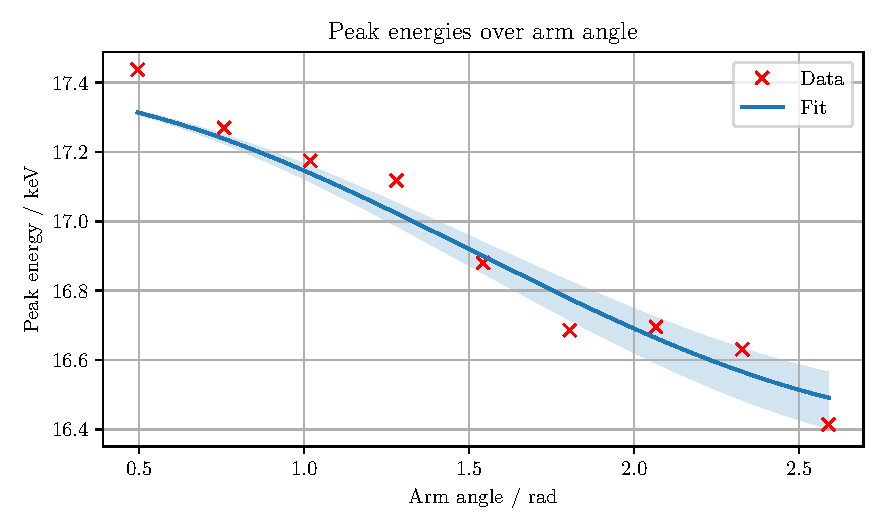
\includegraphics[width=0.95\textwidth]{../plots/energie_winkel.pdf}
        \caption[Gestreute Energie $E_S$ gegen Winkel $\varphi$]{Gestreute Energie $E_S$ aus \autoref{tab:energy_compton} aufgetragen gegen den Winkel $\varphi$ des Messarms. Fitkurve mit $2\sigma$-Unsicherheitband.}
        \label{fig:compton_energy}
    \end{samepage}
\end{figure}


\subsection{Röntgenfluoreszenzanalyse}
\label{subsec:auswertung_fluoreszenz}

Auch für den zweiten Teilversuch liegen die Daten in \texttt{.csv}-Form vor. Diese werden nun in \autoref{fig:roentgenfluoreszenz1} und \autoref{fig:roentgenfluoreszenz2} für die zu untersuchenden Materialien dargestellt. Zusätzlich sind die Energien der bestimmten K$_{\alpha}$- und K$_{\beta}$-Linien ebenfalls in den beiden Abbildungen angeführt.
%
\begin{figure}[H]
    \centering
    \begin{tabular}{cc}
        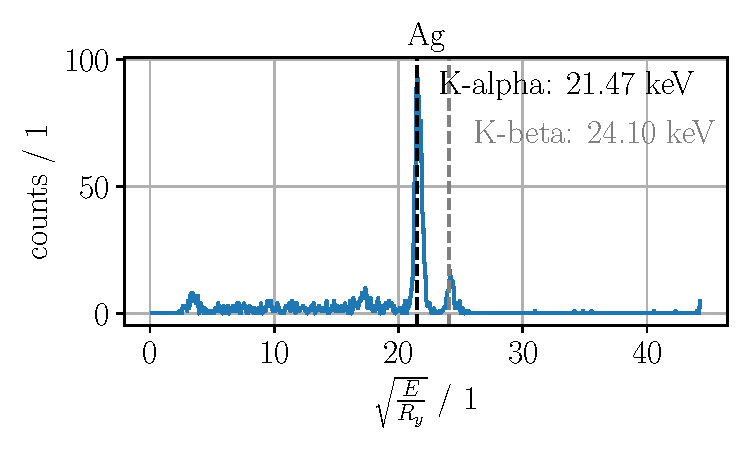
\includegraphics[width=0.48\textwidth]{../plots/roentgen_data_1.pdf} &
        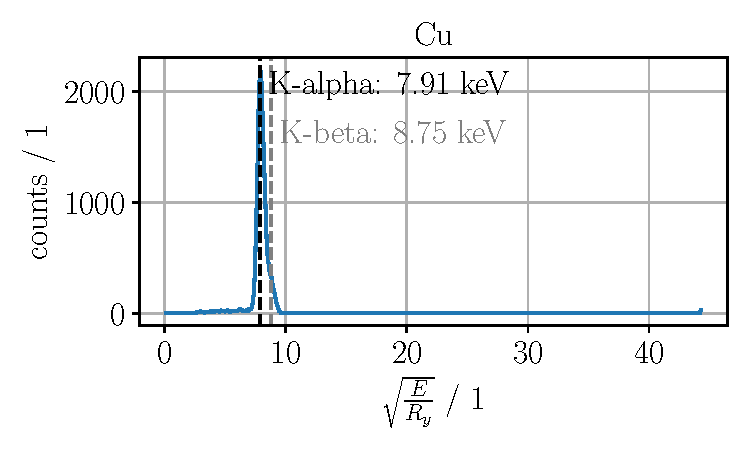
\includegraphics[width=0.48\textwidth]{../plots/roentgen_data_2.pdf}   \\
        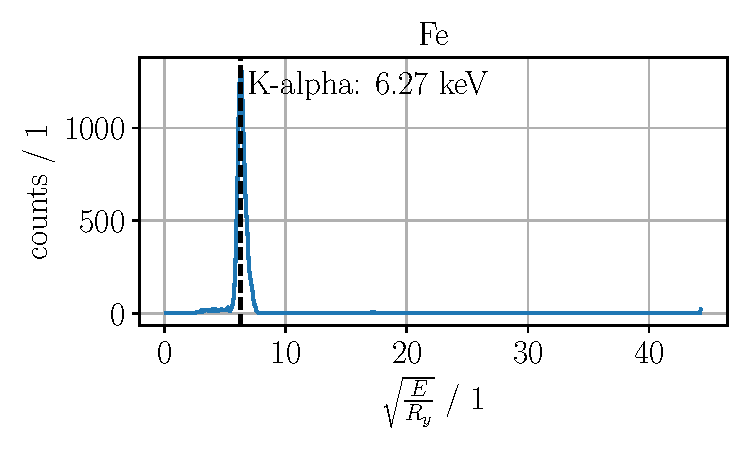
\includegraphics[width=0.48\textwidth]{../plots/roentgen_data_3.pdf} &
        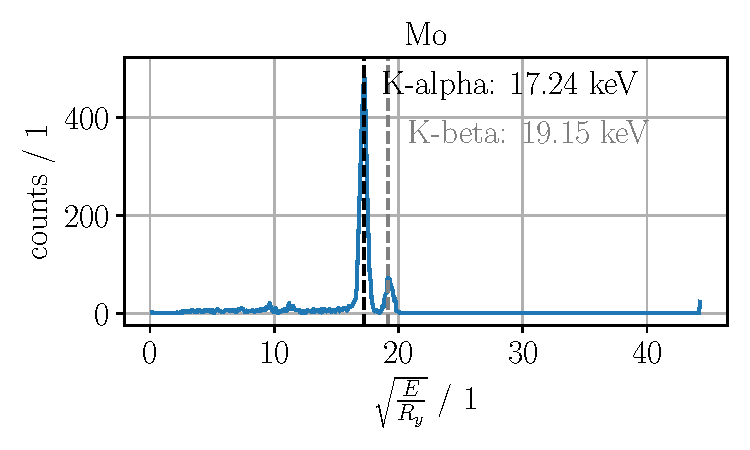
\includegraphics[width=0.48\textwidth]{../plots/roentgen_data_4.pdf}   \\
        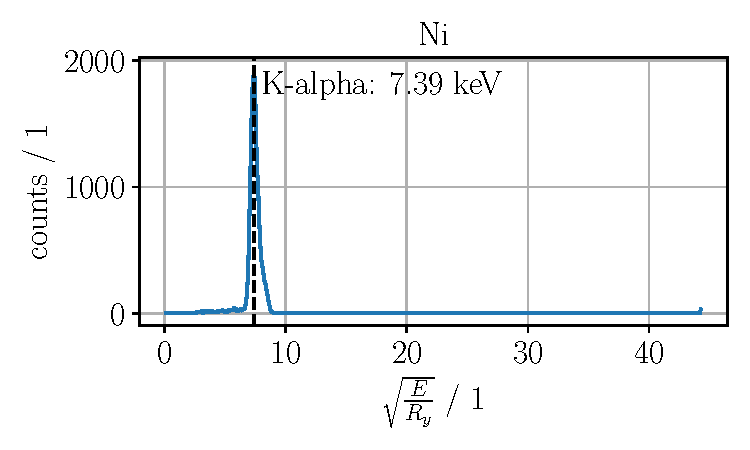
\includegraphics[width=0.48\textwidth]{../plots/roentgen_data_5.pdf} &
        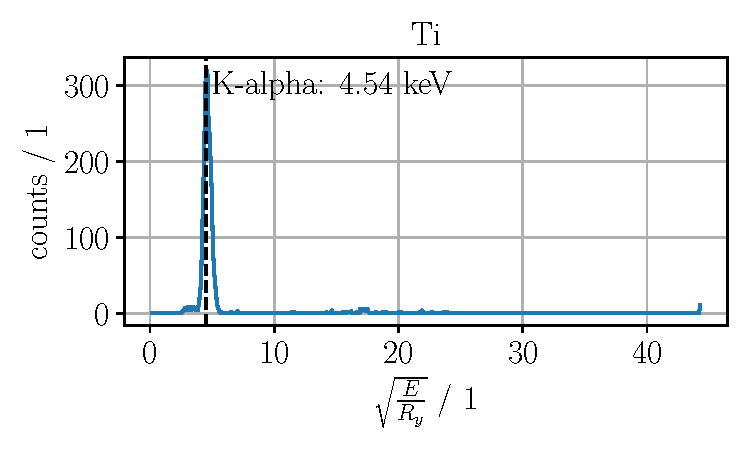
\includegraphics[width=0.48\textwidth]{../plots/roentgen_data_6.pdf}   \\
    \end{tabular}
    \caption[Messwerte unbekannter Proben (1)]{Messwerte und K$_{\alpha}$- und K$_{\beta}$-Linien für die zu untersuchenden bekannten und unbekannten Materialien. (1)}
    \label{fig:roentgenfluoreszenz1}
\end{figure}
%
\begin{figure}[H]
    \centering
    \begin{tabular}{cc}
        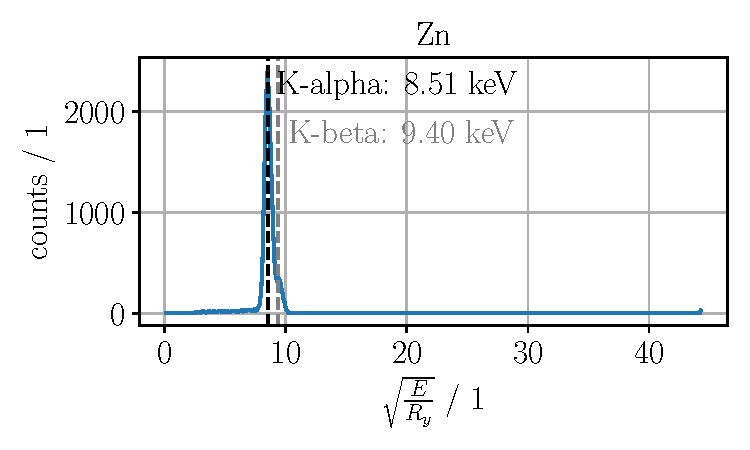
\includegraphics[width=0.48\textwidth]{../plots/roentgen_data_7.pdf}  &
        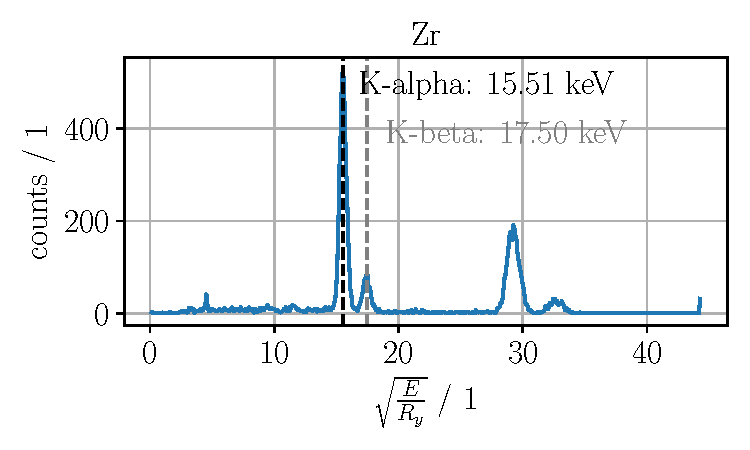
\includegraphics[width=0.48\textwidth]{../plots/roentgen_data_8.pdf}    \\
        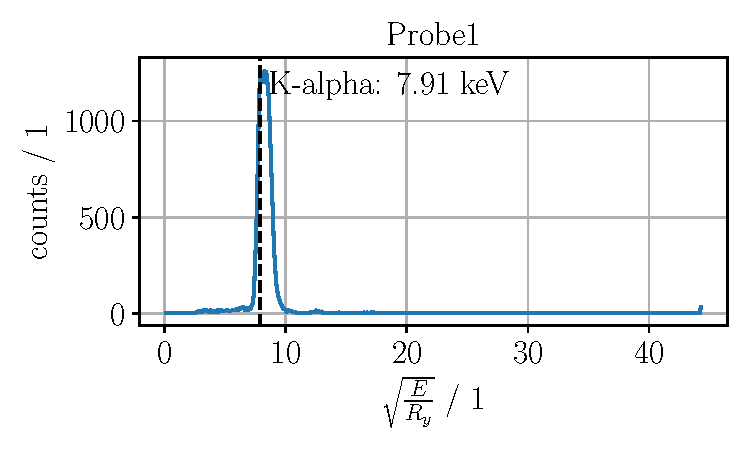
\includegraphics[width=0.48\textwidth]{../plots/roentgen_data_9.pdf}  &
        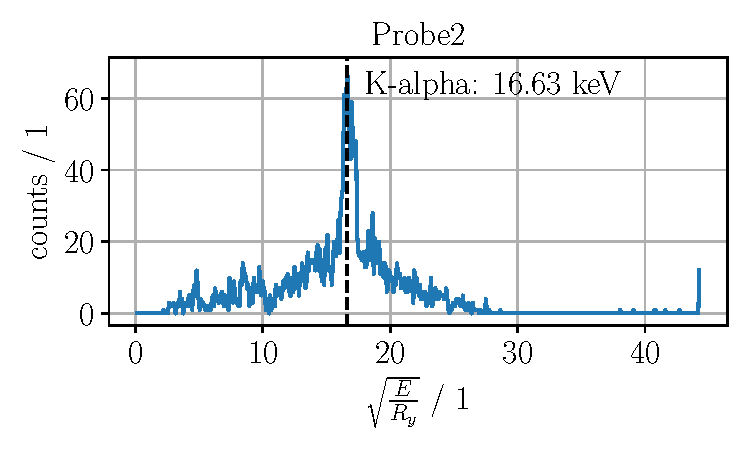
\includegraphics[width=0.48\textwidth]{../plots/roentgen_data_10.pdf}   \\
        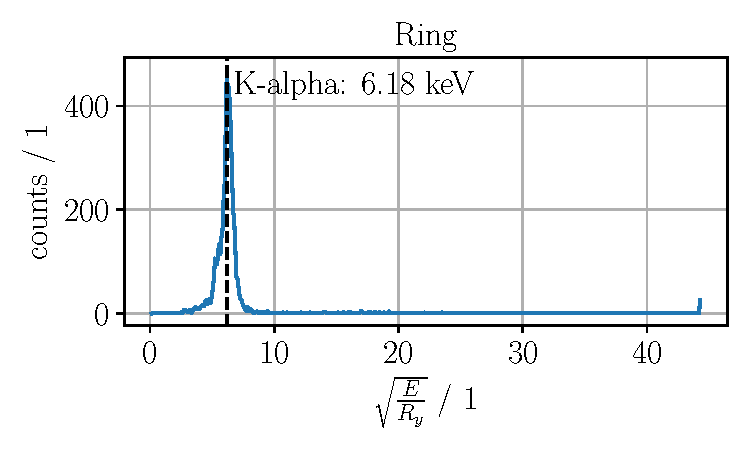
\includegraphics[width=0.48\textwidth]{../plots/roentgen_data_11.pdf} & \\
    \end{tabular}
    \caption[Messwerte unbekannter Proben (2)]{Messwerte und K$_{\alpha}$- und K$_{\beta}$-Linien für die zu untersuchenden bekannten und unbekannten Materialien. (2)}
    \label{fig:roentgenfluoreszenz2}
\end{figure}
%
Die ermittelten Werte für die K$_{\alpha}$- und K$_{\beta}$-Linien werden in \autoref{tab:roentgenfluoreszenz} nochmals angeführt.
%
\begin{table}[H]
    \centering
    \begin{samepage}
        \caption[Bestimmte K$_{\alpha}$- und K$_{\beta}$-Linien]{Bestimmte K$_{\alpha}$- und K$_{\beta}$-Linien aus \autoref{fig:roentgenfluoreszenz1} und \autoref{fig:roentgenfluoreszenz2}. Die Unsicherheit der bestimmten Energien ist in beiden Fällen $\Delta E = \SI{0.1}{\kilo\electronvolt}$.}
        \label{tab:roentgenfluoreszenz}
        \begin{tblr}{colspec={S[table-format=1.0]Q S[table-format=2.2]S[table-format=2.2]}, row{1}={guard}}
            Ordnungszahl & Elementformel & $E_{K_{\alpha}}$ / \si{\kilo\electronvolt} & $E_{K_{\beta}}$ / \si{\kilo\electronvolt} \\
            47           & Ag            & 21.5                                       & 24.1                                      \\
            29           & Cu            & 7.9                                        & 8.8                                       \\
            26           & Fe            & 6.3                                        & {{{-}}}                                   \\
            42           & Mo            & 17.2                                       & 19.2                                      \\
            28           & Ni            & 7.4                                        & {{{-}}}                                   \\
            22           & Ti            & 4.5                                        & {{{-}}}                                   \\
            30           & Zn            & 8.5                                        & 9.4                                       \\
            40           & Zr            & 15.5                                       & 17.5                                      \\
            {{{-}}}      & Probe1        & 7.9                                        & {{{-}}}                                   \\
            {{{-}}}      & Probe2        & 16.6                                       & {{{-}}}                                   \\
            {{{-}}}      & Ring          & 6.2                                        & {{{-}}}                                   \\
        \end{tblr}
    \end{samepage}
\end{table}
%
Trägt man nun die charakteristischen Übergangsenergien aus \autoref{tab:roentgenfluoreszenz} -- leicht modifiziert als $\sqrt{\nicefrac{E}{R_y}}$ -- gegen die Ordnungszahl auf, so kann über die Steigung eines linearen Fits die Abschirmkonstante ermittelt werden. In \autoref{fig:roentgen_z_vs_e} ist dieser Fit für die K$_{\alpha}$-Linien und K$_{\beta}$-Linien dargestellt. Die Abschirmkonstanten für die K$_{\alpha}$-Linien und K$_{\beta}$-Linien wurden somit mit
\[\sigma_{\text{2,1,exp}} = \num{1.06(9)} \]
\[\sigma_{\text{3,1,exp}} = \num{2.14(10)}\]
beziffert.
%
\begin{figure}[H]
    \centering
    \begin{samepage}
        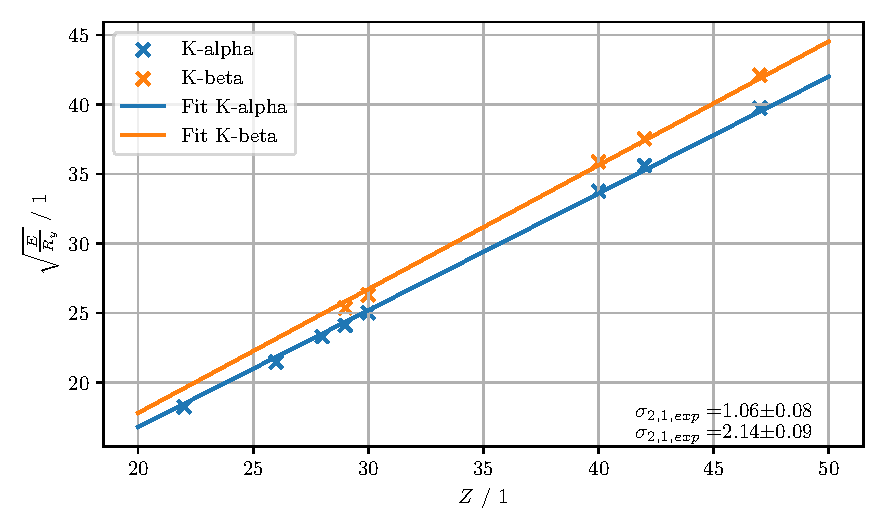
\includegraphics[width=0.95\textwidth]{../plots/roentgen_data_Z_vs_E.pdf}
        \caption[Mosley-Gesetz für die K$_{\alpha}$- und K$_{\beta}$-Linien.]{Moseley-Gesetz für die K$_{\alpha}$- und K$_{\beta}$-Linien. $\sqrt{\nicefrac{E}{R_y}}$ gegen die Ordnungszahl aufgetragen. Die Abschirmkonstante wird aus der Steigung der beiden Fits ermittelt.}
        \label{fig:roentgen_z_vs_e}
    \end{samepage}
\end{figure}


\subsection{Unbekannte Proben}
\label{sec:roentgen_unbekannt}

Nun werden die drei verbleibenden unbekannten Proben untersucht. Die Messungen werden wie in \autoref{subsec:durchfuehrung_compton} durchgeführt und die Ergebnisse der Messungen sind in \autoref{fig:roentgenfluoreszenz2} abgebildet.

Es ergeben sich für die Proben folgenden Werte für die potentiellen K$_{\alpha}^*$-Linien in \autoref{tab:roentgenfluoreszenz_unbekannt}

\begin{table}[H]
    \centering
    \begin{samepage}
        \caption[Bestimmte K$_{\alpha}^*$-Linien unbekannte Proben]{Bestimmte K$_{\alpha}^*$-Linien der unbekannten Proben aus \autoref{fig:roentgenfluoreszenz2}. Die Unsicherheit der bestimmten Energien ist in beiden Fällen $\Delta E = \SI{0.1}{\kilo\electronvolt}$.}
        \label{tab:roentgenfluoreszenz_unbekannt}
        \begin{tblr}{colspec={Q S[table-format=2.2] Q S[table-format=2.2]}, row{1}={guard}}
            Probenname & $E_{K_{\alpha}^*}$ / \si{\kilo\electronvolt} & Potentielles Element & $E_{K_{\alpha}}$ / \si{\kilo\electronvolt} \\
            Probe1     & 7.9                                          & Cu                   & 7.9                                        \\
            Probe2     & 16.6                                         & Mo \footnotemark{}   & 17.2                                       \\
            Ring       & 6.2                                          & Fe                   & 6.3                                        \\
        \end{tblr}
    \end{samepage}
\end{table}
\footnotetext[1]{Molybdän ist zwar von der Energie her das passendste Element für den Peak, jedoch ist es fraglich, ob es sich bei der Probe tatsächlich um Molybdän handelt.}


\section{Diskussion}
\label{sec:diskussion}

\subsection{Compton-Streuung}
\label{sec:diskussion_compton}

%! powered by GPT-4
Die Ergebnisse des Compton-Streuungs-Teilversuchs zeigen, dass die gemessenen Energien der gestreuten Photonen in \autoref{tab:energy_compton} in guter Übereinstimmung mit den theoretischen Erwartungen des Compton-Effekts stehen. Die Abhängigkeit der gestreuten Energie von dem Winkel des Messarms wurde in \autoref{fig:compton_energy} dargestellt, und es zeigt sich eine klare Tendenz, die dem Compton-Effekt entspricht.


\subsection{Röntgenfluoreszenzanalyse}
\label{sec:diskussion_roentgen}
%! powered by GPT-4 & Elias
Die Ergebnisse der Röntgenfluoreszenzanalyse zeigen, dass die gemessenen Energien der K$_{\alpha}$- und K$_{\beta}$-Linien in guter Übereinstimmung mit den theoretischen Erwartungen stehen. Bei genauer Betrachtung der \autoref{fig:roentgen_z_vs_e} erkennt man, dass ein Fit der ersten paar Punkte -- mit Kernladungszahlen $<35$ -- zu einer Gerade mit höherer Steigung führen würde als einer, welcher lediglich durch die Elemente höherer Ordnungszahlen gegeben wäre. Hier spielt der Einfluss der äußeren Elektronen, welche sich mit steigender Schalenzahl immer weiter von dem Kern entfernen, eine Rolle. Die Abschirmkonstante für die K$_{\alpha}$-Linien und K$_{\beta}$-Linien ist eben nur eine Näherung, wie jedoch auch aus der Abbildung ersichtlich wird, für viele Fälle eine gute.

\subsection{Unbekannte Proben}
\label{sec:diskussion_unbekannt}

Die Ergebnisse der Untersuchung der drei unbekannten Proben, die in \autoref{fig:roentgenfluoreszenz2} dargestellt sind, zeigen potentielle K$_{\alpha}^*$-Linien für jede Probe. Die ausgewerteten Werte sind in \autoref{tab:roentgenfluoreszenz_unbekannt} zusammengefasst. Die Unsicherheit der bestimmten Energien beträgt in beiden Fällen $\Delta E = 0,1$ keV.

Probe 1 zeigt eine K${_\alpha}^*$-Linie bei \SI{7.9}{\kilo\electronvolt}, was auf Kupfer (Cu) als potenzielles Element hindeutet, da die Energie der K${_\alpha}$-Linie von Kupfer ebenfalls \SI{7.9}{\kilo\electronvolt} beträgt.

Probe 2 hat eine K$_{\alpha}^*$-Linie bei 16,6 keV, was auf Molybdän (Mo) als mögliches Element hindeutet. Die Energie der K$_{\alpha}$-Linie von Molybdän beträgt jedoch 17,2 keV. Jedoch ist diese Messung eher weniger aussagekräftig, da die über das ganze Energiespektrum weniger Energie streut. Die vorliegende Methode ist somit eher schlechter für die Bestimmung der Zusammensetzung der 2. Probe geeignet.

Der Ring weist eine K$_{\alpha}^*$-Linie bei 6,2 keV auf, was auf Eisen (Fe) als potenzielles Element hindeutet. Die Energie der K$_{\alpha}$-Linie von Eisen beträgt 6,3 keV, was nahe genug an der gemessenen Energie liegt, um Eisen als mögliches Element zu bestätigen.

\section{Zusammenfassung}
\label{sec:zusammenfassung}

%! powered by GPT-4
Im ersten Teilversuch, der Compton-Streuung, wurden die Energien der Compton-Streuung für verschiedene Winkel gemessen. Die Messwerte sind in \autoref{tab:energy_compton} dargestellt. Aus den Messwerten wurde mittels einer Fitkurve in \autoref{fig:compton_energy} die Elektronenmasse bestimmt: $m_e = \SI{1.07(11)E-30}{\kilogram}$. Der Literaturwert der Elektronenmasse beträgt etwa $\SI{9.11E-31}{\kilogram}$, was zeigt, dass der ermittelte Wert in der richtigen Größenordnung liegt.

Im zweiten Teilversuch, der Röntgenfluoreszenzanalyse, wurden die K$_{\alpha}$- und K$_{\beta}$-Linien für verschiedene Elemente und Proben untersucht. Die Messwerte und bestimmten Energien sind in \autoref{tab:roentgenfluoreszenz} aufgeführt. Durch Auftragen von $\sqrt{\nicefrac{E}{R_y}}$ gegen die Ordnungszahl und Anpassung einer linearen Fitkurve in \autoref{fig:roentgen_z_vs_e} wurden die experimentellen Abschirmkonstanten für die K$_{\alpha}$-Linien und K$_{\beta}$-Linien ermittelt: $\sigma_{\text{2,1,exp}} = \num{1.06(9)}$ und $\sigma_{\text{3,1,exp}} = \num{2.14(10)}$. Die ermittelten Abschirmkonstanten zeigen eine gute Übereinstimmung mit den bekannten Literaturwerten, die in der Regel nahe bei 1 und 2 liegen.

\textbf{TODO unbekannte Proben}



\clearpage
% Literaturverzeichnis
\printbibliography

% Abbildungsverzeichnis
\listoffigures

% Tabellenverzeichnis
\listoftables


\end{document}